\documentclass{beamer}
\usetheme{Darmstadt}
\usecolortheme{beaver}
\usepackage{booktabs}
\usepackage{hyperref}

\usepackage[utf8]{inputenc}
\usepackage{graphicx}
\graphicspath{ {./images/} }

%Information to be included in the title page:
\title{Homework 03}
\author{Brandon Hosley}
\institute{University of Illinois - Springfield}
\date{\today}

\begin{document}
\frame{\titlepage}

\begin{frame}{Overview}
\tableofcontents
\end{frame}

\section[Q1]{Q1: Linear Regression}

\begin{frame}{Linear Regression Problem 1: Simplicity}
	\begin{itemize}
		\item[+] Computationally easy
		\item[-] Can only accurately represent simple relationships
		\item[-] Can only accurately represent linear relationships
	\end{itemize}
	\includegraphics[width=0.75\linewidth]{AnscombeQuartet}
\end{frame}

\begin{frame}{Linear Regression Problem 2: Selection Bias}
	Linear regression is susceptible to selection bias
	\begin{itemize}
		\item A type of overfitting
		\item Occurs when a type of data is over-represented in test set
	\end{itemize}
	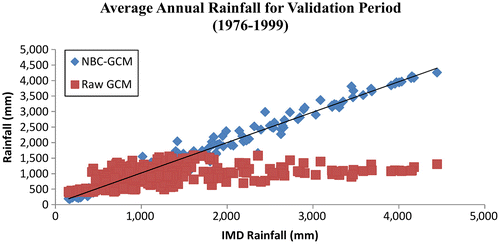
\includegraphics[width=0.45\linewidth]{SelectionBias}
	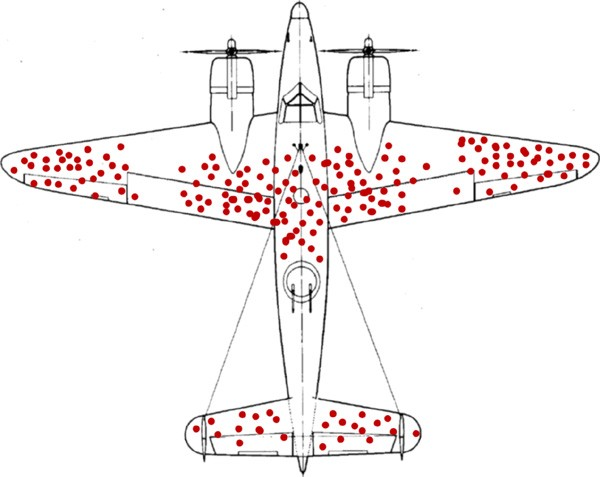
\includegraphics[width=0.45\linewidth]{SelectionAnecdote}
\end{frame}

\begin{frame}{Linear Regression Problem 3: }
	\begin{itemize}
		\item
	\end{itemize}
	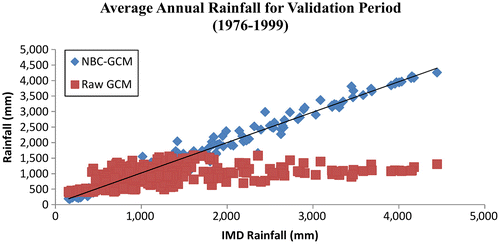
\includegraphics[width=0.75\linewidth]{SelectionBias}
\end{frame}

\begin{frame}{Linear Regression Problem 4: Heteroscedasticity}
	\begin{itemize}
		\item
	\end{itemize}
	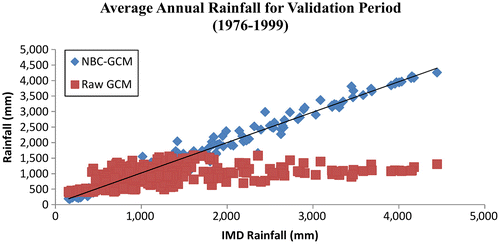
\includegraphics[width=0.75\linewidth]{SelectionBias}
\end{frame}

\section[Q2]{Q2: Hastie and Tibshirani Summary}

\begin{frame}{Hastie Lectures Summary}
	\begin{itemize}
		\item 
	\end{itemize}
\end{frame}


%\section[Q3]{Q3: ISL Section 3.6}
%\section[Q4]{Q4: ISL Section 3.7}
%Exercises. No. 15

\end{document}
